
%(BEGIN_QUESTION)
% Copyright 2007, Tony R. Kuphaldt, released under the Creative Commons Attribution License (v 1.0)
% This means you may do almost anything with this work of mine, so long as you give me proper credit

The following photograph (showing the back side of a control panel) contains so many examples of {\it bad} wiring practice that it is difficult to know where to begin criticism:

$$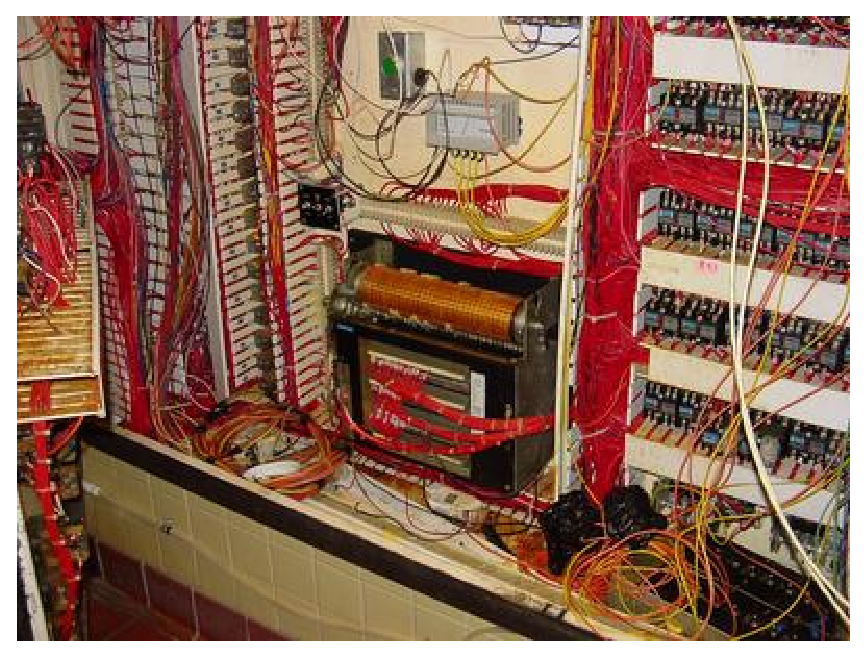
\includegraphics[width=15.5cm]{i02283x01.eps}$$

Identify some of the poor wiring practices in this photograph, trying not to laugh too loudly as you do.

\underbar{file i02283}
%(END_QUESTION)





%(BEGIN_ANSWER)

\begin{itemize}
\item{} Covers left off of many wire ducts.
\item{} It looks like someone didn't even attempt to put some of the wires inside wire ducts, but instead left them draped directly over components.
\item{} In areas where there are no wire ducts, the wires should have been ``loomed'' together instead of randomly strewn.
\item{} Junk items left on the bottom of the cabinet.
\item{} Colored stains on the wire duct (on the left-hand side of the photograph, on the cabinet door) suggest liquid intrusion into the cabinet, most likely from a lack of proper door-to-cabinet sealing.
\end{itemize}

%(END_ANSWER)





%(BEGIN_NOTES)


%INDEX% Good practices, wiring: example of bad wiring

%(END_NOTES)


